\documentclass[12pt,a4paper]{scrartcl}
\usepackage{ifpdf}
\usepackage[utf8]{inputenc}
\usepackage[ngerman]{babel}
\usepackage{amsmath}
\usepackage{amssymb}
\usepackage{fancyhdr}
\usepackage{listings}
\usepackage{color}
\usepackage{pdfpages}
\usepackage{stmaryrd}

\pagestyle{fancy}
\fancyhead{}
\fancyfoot{}
\fancyhead[LO,LE]{Johannes Hedtrich, Christopher Hlubek}
\fancyhead[RO,RE]{Serie 03}
\fancyfoot[CO,CE]{\thepage}

\title{Serie 03}
\author{Johannes Hedtrich, Christopher Hlubek}
\date{\today}
\begin{document}

\section*{3.3}

\subsection*{Voraussetzung:}

Seien $\varphi, \psi$ \emph{einfache Konjunktionen}.

\subsection*{Behauptung:}

Wenn $\textrm{vars}(\varphi) = \textrm{vars}(\psi)$, dann $\varphi \equiv \psi$.

\subsection*{Hilfsbeweis:}

Zeige zuerst folgende Behauptung:\\
Wenn $\rho $ eine \emph{einfache Konjunktion}, dann
\begin{math}
\llbracket \rho\rrbracket^\beta = \begin{cases}
1, & \textrm{falls f.a. }X\in \textrm{vars}(\rho): \beta(X) = 1 \\
0, & \textrm{sonst}
\end{cases}
\end{math}\\
Beweis durch Induktion über $n = l(\rho)$.
\paragraph*{Induktionsanfang:}
\begin{enumerate}
\item $\rho = X_i, i \in \mathbb{N}$. Dann gilt $\llbracket X_i\rrbracket = \beta(X_i)$.
\item $\rho = 1$. Dann ist $\textrm{vars}(\rho) = \emptyset$ und die Behauptung gilt.
\end{enumerate}
\paragraph*{Induktionsschritt:}
\begin{quote}
$\rho = (\varphi \wedge \psi)$ mit $\varphi, \psi$ \emph{einfache Konjunktionen}.
\end{quote}
Es gilt nach Def. $\llbracket (\varphi \wedge \psi)\rrbracket^\beta = 1$ gdw. $\llbracket \varphi\rrbracket^\beta = 1$ und
$\llbracket \psi\rrbracket^\beta = 1$. Nach Induktionsannahme gilt die Behauptung für
$\varphi$ und $\psi$, somit gilt:
\begin{align*}
\llbracket (\varphi \wedge \psi)\rrbracket^\beta
&= \begin{cases}
1, & \textrm{falls f.a. }X\in \textrm{vars}(\varphi): \beta(X) = 1 \textrm{ und } \textrm{f.a. }X\in \textrm{vars}(\psi): \beta(X) = 1\\
0, & \textrm{sonst}
\end{cases}\\
&= \begin{cases}
1, & \textrm{f.a. }X\in \textrm{vars}(\varphi) \cup \textrm{vars}(\psi): \beta(X) = 1 \\
0, & \textrm{sonst}
\end{cases}\\
&= \begin{cases}
1, & \textrm{f.a. }X\in \textrm{vars}((\varphi \wedge \psi)): \beta(X) = 1 \\
0, & \textrm{sonst}
\end{cases}
\end{align*}\\
Daraus folgt die Behauptung des Hilfsbeweises.

\subsection*{Beweis:}

Annahme: $\textrm{vars}(\varphi) = \textrm{vars}(\psi)$. Sei $\beta$ eine Belegung, die zu
$\varphi$ und $\psi$ passt.

\begin{align}
\llbracket \varphi\rrbracket^\beta
&= \begin{cases}
1, & \textrm{f.a. }X\in \textrm{vars}(\varphi): \beta(X) = 1\\
0, & \textrm{sonst}
\end{cases}\\
&= \begin{cases}
1, & \textrm{f.a. }X\in \textrm{vars}(\psi): \beta(X) = 1\\
0, & \textrm{sonst}
\end{cases}\\
&= \llbracket \psi\rrbracket^\beta
\end{align}\\

\begin{enumerate} 
\item Nach Hilfsbeweis
\item Da $\text{vars}(\varphi) = \text{vars}(\psi)$ nach Annahme
\item Nach Hilfsbeweis
\end{enumerate} 

Somit gilt $\varphi \equiv \psi$. $\blacksquare$

\section*{3.4}
 
\subsection*{Voraussetzung:}

Seien $\varphi, \psi, \chi, \rho \in F_{AL}$.

\subsection*{Behauptung:}

$((\varphi \wedge \psi) \wedge \chi) \rightarrow \rho \equiv \varphi
\rightarrow (\psi \rightarrow (\chi \rightarrow \rho))$

\subsection*{Beweis:}
\setcounter{equation}{0}
\begin{align}
  ((\varphi \wedge \psi) \wedge \chi) \rightarrow \rho
  	& \equiv \neg((\varphi \wedge \psi) \wedge \chi) \vee \rho \\
  	& \equiv (\neg(\varphi \wedge \psi) \vee \neg\chi) \vee \rho \\
  	& \equiv ((\neg\varphi \vee \neg\psi) \vee \neg\chi) \vee \rho \\
  	& \equiv (\neg\varphi \vee (\neg\psi \vee \neg\chi)) \vee \rho \\
  	& \equiv \neg\varphi \vee (\neg\psi \vee (\neg\chi \vee \rho)) \\
  	& \equiv \neg\varphi \vee (\neg\psi \vee (\chi \rightarrow \rho)) \\
  	& \equiv \neg\varphi \vee (\psi \rightarrow (\chi \rightarrow \rho)) \\
  	& \equiv \varphi \rightarrow (\psi \rightarrow (\chi \rightarrow \rho))
\end{align}

O.B.d.A. gelte im Folgenden $X_0 \not\in \textrm{vars}(\varphi) \cup \textrm{vars}(\psi) \cup \textrm{vars}(\chi) \cup \textrm{vars}(\rho)$.

\begin{enumerate} 
\item Konditional Elimination 
\item 2. Ersetzungslemma:
$i = 0$, $\varphi_s = X_0 \vee \rho$, $\psi_s = \neg((\varphi \wedge \psi) \wedge \chi)$, $\psi'_s = (\neg(\varphi \wedge \psi) \vee \neg\chi)$.
$\psi_s \equiv \psi'_s$ gilt nach De Morgan.
\item 2. Ersetzungslemma:
$i = 0$, $\varphi_s = (X_0 \vee \neg\chi) \vee \rho$, $\psi = \neg(\varphi \wedge \psi)$, $\psi'_s = (\neg\varphi \vee \neg\psi)$.
$\psi_s \equiv \psi'_s$ gilt nach De Morgan.
\item Assoziativität von $\vee$
\item Assoziativität von $\vee$
\item 2. Ersetzungslemma:
$i = 0$, $\varphi_s = \neg\varphi \vee (\neg\psi \vee X_0)$, $\psi_s = \neg\chi \vee \rho$, $\psi'_s = \chi \rightarrow \rho$.
$\psi_s \equiv \psi'_s$ gilt nach Konditional-Regel.
\item 2. Ersetzungslemma:
$i = 0$, $\varphi_s = \neg\varphi \vee X_0$, $\psi_s = \neg\psi \vee (\chi \rightarrow \rho)$, $\psi'_s = \psi \rightarrow (\chi \rightarrow \rho)$.
$\psi_s \equiv \psi'_s$ gilt nach Konditional-Regel.
\item Konditional-Regel
\end{enumerate}

$\blacksquare$

\section*{3.5}

Kodierung eines Literals $X_{i,j}^k$: $X_{ijk}$, also für $X_{12}^3$ zu $X_{123}$.

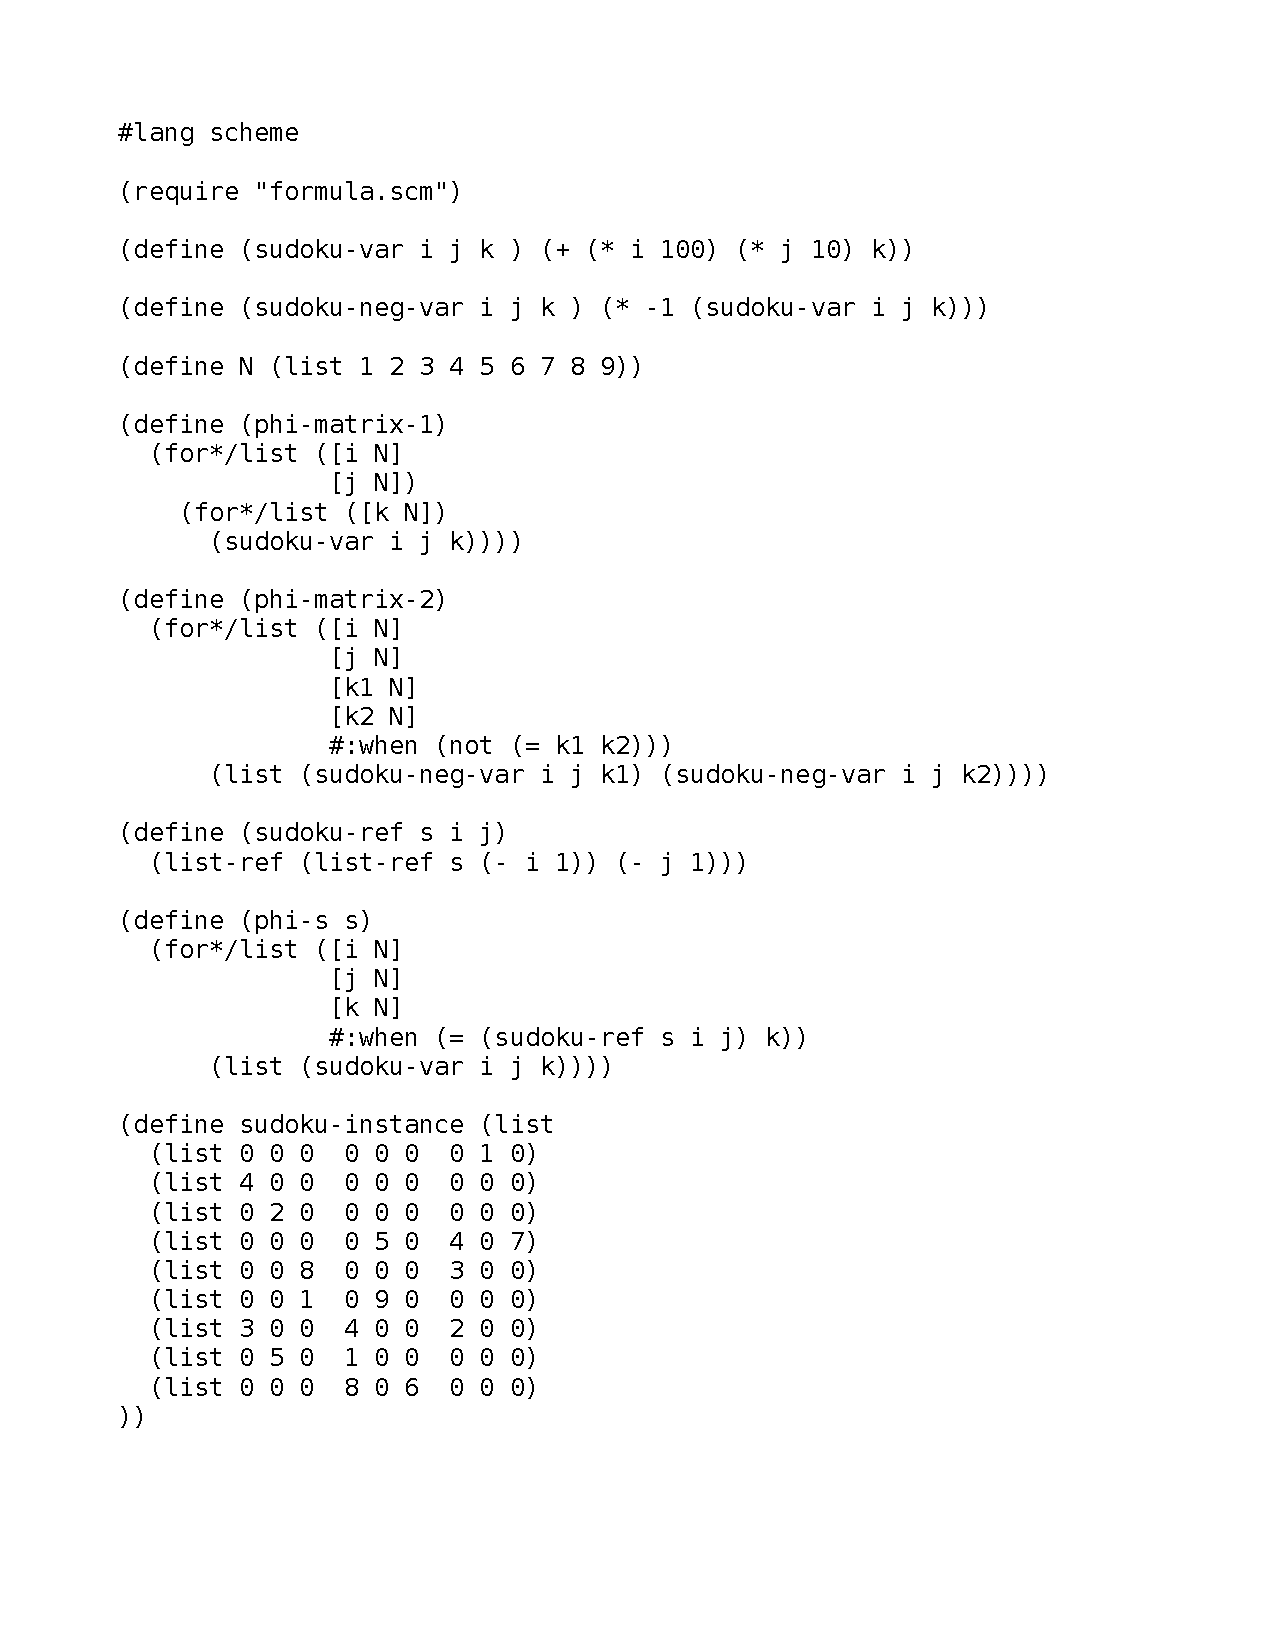
\includepdf[pages=-]{sudoku.pdf}

\end{document}
